
\subsection{Tableaux Semânticos}

\begin{frame}[t]

\vskip 3cm

\begin{center}
{\Huge Tableaux Semânticos}
\end{center}

\end{frame}


\begin{frame}{Definição:}
Sistema de dedução que possui uma estrutura que permite a representação e a dedução formal de conhecimento. Por não ser axiomático os tableaux semânticos são mais adequados para implementações em computadores.
\vspace{0,7 cm}

Diferente dos outros métodos, os tableaux semânticos estabelecem um importante mecanismo de decisão, pois, nos permitem inferir a falsidade da consequência sintática.
\end{frame}

\begin{frame}{Elementos Básicos}
\begin{itemize}
\item O alfabeto da Lógica Proposicional
\item O conjunto das fórmulas da Lógica Proposicional
\item Um conjunto de regras de dedução
\end{itemize}
\vspace{0,7 cm}
Os elementos básicos do sistema de tableaux semânticos determinam a sua estrutura. Os tableaux semânticos contém apenas regras de dedução que definem o mecanismo de inferência.
\end{frame}

\begin{frame}{Regras de Inferências}
\begin{itemize}
\item Regras de Inferência que Prolongam:\\
\vspace{0,7 cm}

\begin{tikzpicture}
{\tiny 
\path (1,3) node (1) {$R_1:$};
\path (2,2) node (2) {$p \wedge q$};
\path (2,1) node (3) {p};
\path (2,0) node (4) {q};
\path (4,3) node (5) {$R_5:$};
\path (5,2) node (6) {$\sim \sim p$};
\path (5,1) node (7) {p};
\path (7,3) node (8) {$R_7:$};
\path (8,2) node (9) {$\sim(p \vee q)$};
\path (8,1) node (10) {$\sim p$};
\path (8,0) node (11) {$\sim q$};
\path (10,3) node (12) {$R_8:$};
\path (11,2) node (13) {$\sim(p\rightarrow q)$};
\path (11,1) node (14) {p};
\path (11,0) node (15) {$\sim q$};

\draw (2) -- (3) ;
\draw (3) -- (4) ;
\draw (6) -- (7) ;
\draw (9) -- (10) ;
\draw (10) -- (11) ;
\draw (13) -- (14) ;
\draw (14) -- (15) ;
}

\end{tikzpicture}
\end{itemize}
\end{frame}

\begin{frame}{Regras de Inferências - Continuação}
\begin{itemize}
\item Regras de Inferência que Bifurcam:\\
\vspace{0,7 cm}

\begin{tikzpicture}
{\tiny 
\path (1,6) node (1) {$R_2$:};
\path (2,5) node (2) {$p \vee q$};
\path (1,4) node (3) {$p$};
\path (3,4) node (4) {$q$};
\path (5,6) node (5) {$R_3:$};
\path (6,5) node (6) {$p \rightarrow q$};
\path (5,4) node (7) {$\sim p$};
\path (7,4) node (8) {$q$};
\path (9,6) node (9) {$R_4:$};
\path (10,5) node (10) {$p \leftrightarrow q$};
\path (9,4) node (11) {$p \wedge q$};
\path (11,4) node (12) {$\sim p \wedge \sim q$};
\path (1,3) node (13) {$R_6:$};
\path (2,2) node (14) {$ \sim (p \wedge q$)};
\path (1,1) node (15) {$ \sim p$};
\path (3,1) node (16) {$\sim q$};
\path (5,3) node (17) {$R_9:$};
\path (6,2) node (18) {$ \sim (p \leftrightarrow q)$};
\path (5,1) node (19) {$ \sim p \wedge q$};
\path (7,1) node (20) {$p \wedge \sim q$};

\draw (2) -- (3) ;
\draw (2) -- (4) ;
\draw (6) -- (7) ;
\draw (6) -- (8) ;
\draw (10) -- (11) ;
\draw (10) -- (12) ;
\draw (14) -- (15) ;
\draw (14) -- (16) ;
\draw (18) -- (19) ;
\draw (18) -- (20) ;
}
\end{tikzpicture}
\end{itemize}
\end{frame}

\begin{frame}{Aplicação do Método de Prova no sistema dos Tableaux Semânticos}
O método de prova nos tableaux semânticos é feita utilizando o método da negação ou redução ao absurdo. Dessa forma, para provar uma fórmula $H$, inicialmente consideramos $\sim H$. \\ Em seguida precisamos:

\begin{itemize}
\item Construir o tableau semântico para $\sim H$.
\item Utilizando as regras de dedução, a fórmula $\sim H$ é decomposta em subfórmulas.
\end{itemize}
\end{frame}

\begin{frame}{Construção de um Tableau Semântico}
Um tableau semântico na Lógica Proposicional, é construído como segue:\\
\vspace{0,7 cm}
Seja um conjunto de fórmulas $$\{ A_1,..., A_n\} $$
\end{frame}

\begin{frame}{Exemplo de construção de um tableau semântico}
Considere o conjunto de fórmulas:\\
$$\{ (p \vee q),(p \wedge \sim q)\}$$
\centering

\begin{tikzpicture}
\path (3,4) node (1) {1:};
\path (5,4) node (2) {$p \vee q$};
\path (3,3) node (3) {2:};
\path (5,3) node (4) {$p \wedge \sim q$};
\path (3,2) node (5) {3:};
\path (5,2) node (6) {p};
\path (8,2) node (7) {$R_1,2.$};
\path (3,1) node (8) {4:};
\path (5,1) node (9) {$\sim q$};
\path (8,1) node (10) {$R_1,2.$};
\path (3,0) node (11) {5:};
\path (4,0) node (12) {$p$};
\path (6,0) node (13) {$q$};
\path (8,0) node (14) {$R_2,1.$};

\draw (2) -- (4) ;
\draw (4) -- (6) ;
\draw (6) -- (9) ;
\draw (9) -- (12) ;
\draw (9) -- (13) ;
\end{tikzpicture}

\vspace{0,7 cm}
\begin{itemize}
\item Heurística (Aplicação de regras): Aplicamos preferencialmente as regras que prolongam.
\end{itemize}
\end{frame}

\begin{frame}{Construção de um Tableau Semântico}
Considere o conjunto de fórmulas
$$\{(p \rightarrow q),\sim(p \vee q), \sim(r \rightarrow p)\}$$

As fórmulas anteriores resultam num tableau que é uma árvore de um ramo só.

\vspace{0,7 cm}
\centering
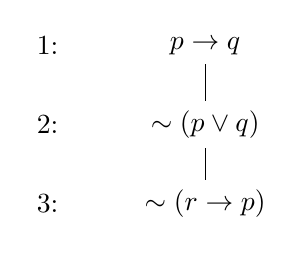
\begin{tikzpicture}
\path (3,2) node (1) {1:};
\path (5,2) node (2) {$p \rightarrow q$};
\path (3,1) node (3) {2:};
\path (5,1) node (4) {$\sim(p \vee q)$};
\path (3,0) node (5) {3:};
\path (5,0) node (6) {$\sim(r \rightarrow p)$};
\draw (2) -- (4) ;
\draw (4) -- (6) ;
\end{tikzpicture}   \\
\vspace{0,7 cm}
\begin{itemize}
\item Aplicando as regras de inferência o tableau resultante será:
\end{itemize}
\end{frame}

\begin{frame}{Tableau Semântico Resultante}
\centering
\begin{tikzpicture}

\path (3,7) node (1) {1:};
\path (5,7) node (2) {$p \rightarrow q$};
\path (3,6) node (3) {2:};
\path (5,6) node (4) {$\sim(p \vee q)$};
\path (3,5) node (5) {3:};
\path (5,5) node (6) {$\sim(r \rightarrow p)$};
\path (3,4) node (7) {4:};
\path (5,4) node (8) {$\sim p $};
\path (3,3) node (9) {5:};
\path (5,3) node (10) {$\sim q $};
\path (3,2) node (11) {6:};
\path (4,2) node (12) {$\sim p $};
\path (6,2) node (13) {$\sim q $};
\path (8,2) node (14) {$R_3,1.$};
\path (8,3) node (15) {$R_7,2.$};
\path (8,4) node (16) {$R_7,2.$};
\path (3,1) node (17) {7:};
\path (4,1) node (18) {$r$};
\path (6,1) node (19) {$r$};
\path (8,1) node (20) {$R_8,3.$};
\path (3,0) node (21) {8:};
\path (4,0) node (22) {$\sim p$};
\path (6,0) node (23) {$\sim p$};
\path (8,0) node (24) {$R_8,3.$};
\draw (2) -- (4) ;
\draw (4) -- (6) ;
\draw (6) -- (8) ;
\draw (8) -- (10) ;
\draw (10) -- (12) ;
\draw (10) -- (13);
\draw (12) -- (18);
\draw (13) -- (19);
\draw (18) -- (22);
\draw (19) -- (23);
\end{tikzpicture}   
\end{frame}
\begin{frame}{}
O tableau da figura anterior contém dois ramos. Nesse caso, o ramo à direita contém as fórmulas $\sim q$ e $q$. O ramo à esquerda não contém nenhuma fórmula juntamente com sua negação. Essa é uma propriedade a ser identificada nos ramos de um tableau.
\begin{itemize}
\item Ramo: é uma sequência de fórmulas $H_1,...,H_n$ onde $H_1$ é a primeira fórmula do tableau e, nessa sequência, $H_{i+1}$ é a derivada de $H_i$.
\item Ramo Fechado: é fechado se ele contém uma fórmula $H$ e sua negação $\sim H$.
\item Ramo Aberto: é aberto se ele não é fechado.
\end{itemize}
\end{frame}
\begin{frame}
	\begin{itemize}
	    \item Ramo Saturado: é saturado se para toda fórmula $H$, do ramo:
			\begin{itemize}
       	\item já foi aplicada alguma regra de inferência, ou seja, $H$ já   			  foi expandida por alguma regra; ou
	    \item não é possível aplicar nenhuma regra de inferência.
    \end{itemize}
    	\item Tableau Fechado: é fechado quando todos os seus ramos são         	      fechados
        \item Tableau Aberto: é aberto se ele possui algum ramo aberto.
    \end{itemize}
\end{frame}
\begin{frame}{Consequência Lógica no Sistema de Tableaux Semânticos}

Seja $H$ uma fórmula. Uma prova de $H$, no sistema $Tb_a$, é um tableau fechado iniciado com a fórmula $\sim H$. Nesse caso, $H$ é um teorema do sistema de tableax semânticos $Tb_a$.\\
\vspace{0,7 cm}
Considere a fórmula: $$H = \sim((p \rightarrow q) \wedge \sim (p \leftrightarrow q)\wedge \sim \sim p).$$
Observe que o tableau é iniciado com a negação da fórmula $H$, que é igual a
$$\sim \sim((p \rightarrow q) \wedge \sim (p \leftrightarrow q)\wedge \sim \sim p).$$
\\

Após a aplicação das regras, se todos os seus ramos são fechados, o tableaux é fechado, portanto constitui uma prova de $H$.
\end{frame}

\begin{frame}{Exemplo de Aplicação do Sistema de Tableaux Semânticos}

\centering

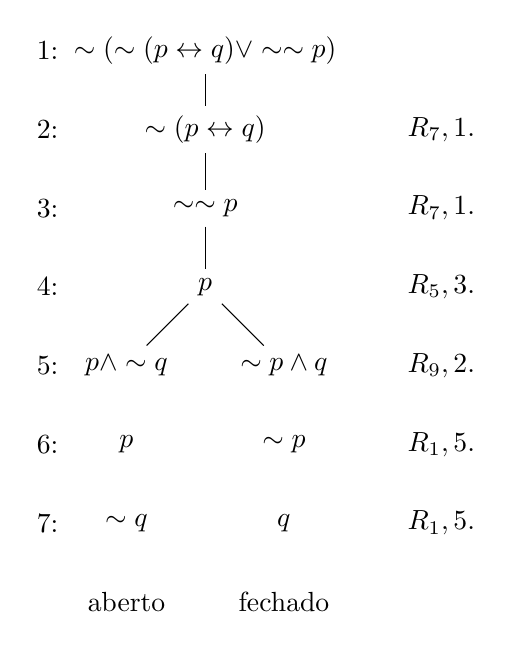
\begin{tikzpicture}
\path (3,7) node (1) {1:};
\path (5,7) node (2) {$ \sim ( \sim (p \leftrightarrow q) \vee \sim \sim p) $};
\path (8,6) node (3) {$R_7,1.$};
\path (3,6) node (4) {2:};
\path (5,6) node (5) {$ \sim (p \leftrightarrow q)$};
\path (8,5) node (6) {$R_7,1.$};
\path (3,5) node (7) {3:};
\path (5,5) node (8) {$\sim \sim p$};
\path (8,4) node (9) {$R_5,3.$};
\path (3,4) node (10) {4:};
\path (5,4) node (11) {$p$};
\path (8,3) node (12) {$R_9,2.$};
\path (3,3) node (13) {5:};
\path (4,3) node (14) {$p \wedge \sim q$};
\path (6,3) node (15) {$\sim p \wedge q$};
\path (8,2) node (16) {$R_1,5.$};
\path (3,2) node (17) {6:};
\path (4,2) node (18) {$p$};
\path (6,2) node (19) {$\sim p$};

\path (8,1) node (20) {$R_1,5.$};
\path (3,1) node (21) {7:};
\path (4,1) node (22) {$ \sim q$};
\path (6,1) node (23) {$q$};

\path (4,0) node (24) {aberto};
\path (6,0) node (25) {fechado};

\draw (2) -- (5) ;
\draw (5) -- (8) ;
\draw (8) -- (11) ;
\draw (11) -- (14);
\draw (11) -- (15);

\end{tikzpicture}
\end{frame}

